\documentclass[12pt]{article}
\usepackage{graphicx} % Required for inserting images
\usepackage{enumitem}
\usepackage{amsmath}
\usepackage{gvv-book}
\usepackage{gvv}

\title{\textbf{4.5.6}}
\author{\textbf{EE25BTECH11004 - Aditya Appana}}
\date{September 12, 2025}

\begin{document}

\maketitle

\section*{Question}
Find the equations of the line that passes through the point (3,0,1) and parallel to the
planes $x + 2y = 0$ and $3y$ $-$ $z = 0$.

\section*{Solution}

We know that the normal form of a plane is $\vec{n}^T\vec{x} = 0$ \\
The plane $x + 2y = 0$ can be expressed in vector form as:
\begin{align}
    \myvec{1\\2\\0}^T\vec{x} = 0
\end{align} 

therefore, \begin{align}\vec{n}_1 = \myvec{1\\2\\0}\end{align} \\
The plane $3y$ $-$ $z=0$ can be expressed in vector form as:

\begin{align}
    \myvec{0 \\ 3 \\-1}^T\vec{x} = 0
\end{align}

therefore, \begin{align}\vec{n}_2 = \myvec{0\\3\\-1} \end{align}

The direction vector of the line is given by:
\begin{align}
\myvec{ 1&2&0 \\ 0&3&-1}\vec{m} = 0 
\end{align}

\begin{align}
\myvec{ 1&2&0 \\ 0&3&-1}\vec{m} = 0 \xrightarrow{\text{R_1 \rightarrow $R_1- \frac{2}{3}R_2$}} \myvec{1&0&\frac{2}{3} \\ 0&3&-1} \xrightarrow{\text{R_1 \rightarrow $R_1/3$}} \myvec{1&0&\frac{2}{3} \\ 0 & 1 & \frac{-1}{3}} 
\end{align}

\begin{align}
\vec{m}= \myvec{-2\\1\\3}
\end{align}

Therefore the equation of the line is:
\begin{align}
\vec{x} = \myvec{3\\0\\1} + \lambda\myvec{-2\\1\\3}
\end{align}

\begin{figure}[H]
    \centering
    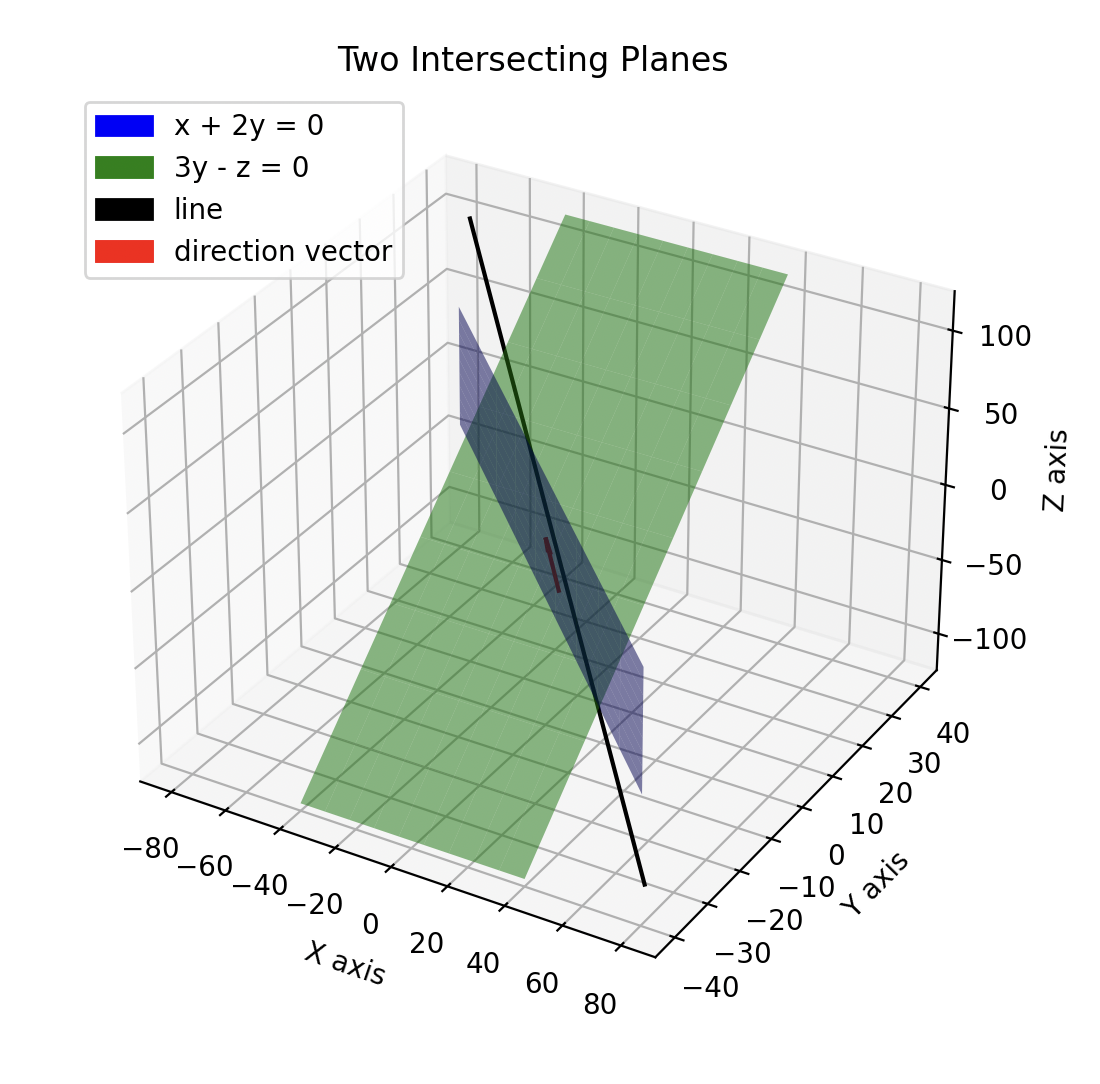
\includegraphics[width=0.9\columnwidth]{Figs/Plot7.png}
    \caption{Plot}
    \label{fig:placeholder}
\end{figure}
\end{document}